\documentclass[10pt]{article}
\usepackage{icmlko}

\icmlmeta{IP 파운데이션 월드모델}{217}{우위가 아니라 결손이었다}{노트 215가 ``공유가 죽인다''고 적었는데 갈라 보니 공유의 정체가 아니었다. 그리고 챔피언의 유일한 손잡이는 살아남았다}

\begin{document}

\twocolumn[
\icmlheader

\begin{abstract}
노트 215가 ``합치는 것이 죽이는 게 아니라 공유가 죽인다''로 스물다섯 노트짜리
물음을 닫았다. 갈랐다 --- \textbf{공유의 정체가 아니다.} 바탕 무리를 키워
가며 그 위에 달력을 얹으면 트리 우위가 바탕 없음 $+$0.0904 · 바탕
위키·검색($\rho$ 0.265) $+$0.0750 · 바탕 공유($\rho$ 0.372) $+$0.0154 ·
바탕 공유$+$위키·검색($\rho$ 0.425) $+$0.0108 이고, \textbf{바탕 $\rho$
와의 상관이 $-$0.975} 다. 공유가 특별한 것이 아니라 \emph{제일 큰} 것이다
(단독 $\rho$ 가 공유 0.372 · 위키·검색 0.265 · 달력 0.013). 그리고 더
날카로운 것이 그 옆에 있었다. 같은 표를 능형과 트리로 나눠 보면
\textbf{능형이 달력에서 얻는 것이 $-$0.0209 $\sim$ $+$0.0133 으로 사실상
0 이다} --- 바탕이 공유일 때 $+$0.0009, 공유$+$위키·검색일 때 $+$0.0041.
그래서 \textbf{트리의 ``우위''는 달력이 그 바탕 위에 더할 수 있는 증분
\emph{전체}}다(이득 $\div$ 트리 증분 $=$ 0.72$\sim$1.39, 평균 0.98).
\textbf{트리가 잘해서가 아니라 능형이 못해서다} --- 노트 186이 ``부호
이질성과 비단조''로 설명한 것의 크기가 이것이다. 그러면 ``달력이 왜
트리에서만 되는가''의 최종 답은 두 줄이다: \textbf{능형은 주기 열에서
아무것도 못 뽑고, 트리가 뽑는 양은 바탕이 이미 얼마나 맞히느냐로 정해진다.}
그리고 노트 216이 남긴 제일 큰 줄을 쟀다 --- \textbf{챔피언 F21 의 유일하게
살아 있는 손잡이(도메인별 풀링 선택)는 안정하다.} 안쪽 분할 지점을 다섯 번
옮겨도 \textbf{열 도메인 전부 3/5 이상이고 여덟이 5/5} 다. 안쪽 격차의
부호도 안 바뀐다 --- 도서 $+$0.09$\sim$$+$0.14 · 모바일 $+$0.027$\sim$
$+$0.037 이 늘 혼자고, 웹툰 $-$0.057$\sim$$-$0.145 · 애니 $-$0.017$\sim$
$-$0.050 이 늘 풀링이다. \textbf{노트 216의 잣대가 변별한다} --- 같은
잣대가 손잡이 둘을 죽이고 이 하나를 통과시킨다.
\end{abstract}
]

\begin{figure*}[t]
\centering
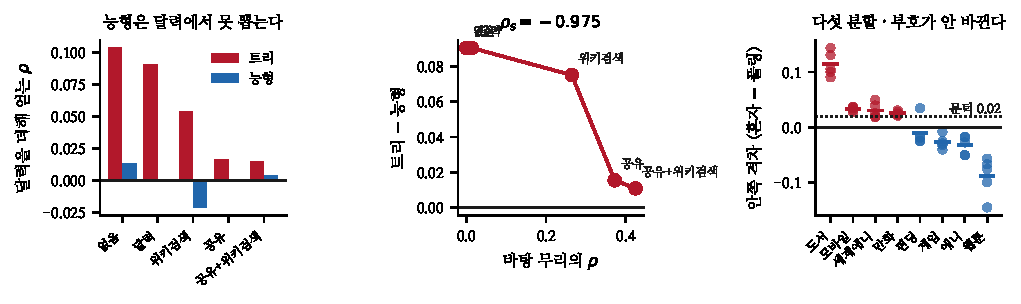
\includegraphics[width=\textwidth]{figs/deficit.pdf}
\caption{왼쪽 --- 능형은 달력에서 못 뽑는다. 가운데 --- 바탕이 크면 남는
것이 없다. 오른쪽 --- 챔피언의 손잡이는 부호가 안 바뀐다.}
\end{figure*}

\section{공유의 정체가 아니었다}

\begin{table}[t]
\centering\tsize
\caption{바탕 무리 위에 달력을 얹으면.}
\begin{tabular}{lrrr}
\toprule
바탕 & 바탕 $\rho$ & 트리$-$능형 \\
\midrule
없음 & .0000 & $+$.0904 \\
달력 & .0133 & $+$.0904 \\
위키·검색 & .2645 & $+$.0750 \\
\textbf{공유} & \textbf{.3723} & \textbf{$+$.0154} \\
공유$+$위키·검색 & .4247 & $+$.0108 \\
\midrule
\multicolumn{2}{l}{바탕 $\rho$ 와의 상관} & \textbf{$-$.975} \\
\bottomrule
\end{tabular}
\end{table}

\claimx{\textbf{공유가 특별한 것이 아니라 제일 큰 것이다.} 단독 $\rho$ 가
공유 0.372 · 위키·검색 0.265 · 달력 0.013 이고, 트리 우위는 바탕 $\rho$ 를
따라 단조로 준다($-$0.975).}{노트 215가 ``공유가 죽인다''고 적은 것은
\emph{맞는 관찰이고 틀린 까닭}이다. 위키·검색을 바탕으로 놔도 $+$0.0750
으로 이미 준다 --- 공유는 더 큰 바탕일 뿐이다.}

\section{능형이 못 뽑는 것}

\begin{table}[t]
\centering\tsize
\caption{달력을 얹어 각자 얻는 증분.}
\begin{tabular}{lrrr}
\toprule
바탕 & 능형 & 트리 & 이득$\div$트리 \\
\midrule
없음 & $+$.0133 & $+$.1036 & 0.87 \\
달력 & $+$.0000 & $+$.0903 & 1.00 \\
위키·검색 & \textbf{$-$.0209} & $+$.0541 & 1.39 \\
공유 & \textbf{$+$.0009} & $+$.0163 & 0.94 \\
공유$+$위키·검색 & \textbf{$+$.0041} & $+$.0149 & 0.72 \\
\bottomrule
\end{tabular}
\end{table}

\claimx{\textbf{능형이 달력에서 얻는 것이 사실상 0 이다}($-$0.021$\sim$
$+$0.013). 그래서 트리의 ``우위''는 달력이 더하는 증분 \emph{전체}가 된다
(평균 0.98).}{\textbf{우위가 아니라 결손이다.} 노트 186이 ``부호 이질성
(일관성 0.542)과 비단조''로 설명한 것의 크기가 이것이다 --- 설명은
맞았고 이 노트는 그 크기를 준다.}

\claimx{\textbf{``달력이 왜 트리에서만 되는가''의 최종 답은 두 줄이다.}
① 능형은 주기 열에서 아무것도 못 뽑는다. ② 트리가 뽑는 양은 바탕이 이미
얼마나 맞히느냐로 정해진다.}{스물다섯 노트가 이것을 못 닫은 까닭은
\emph{한 무리만 놓고} 쟀기 때문이다 --- 거기서는 ②가 안 보인다. \textbf{바탕을
바꿔 가며 재는 한 칸이 없었다.}}

\section{챔피언의 손잡이는 살아남았다}

\begin{table}[t]
\centering\tsize
\caption{안쪽 분할 지점을 0.60$\sim$0.80 으로 다섯 번 옮기면.}
\begin{tabular}{lrl}
\toprule
& 안쪽 격차 & 다섯 분할 \\
\midrule
\textbf{도서} & $+$.09$\sim$$+$.14 & \textbf{혼자 5/5} \\
모바일 & $+$.027$\sim$$+$.037 & 혼자 5/5 \\
만화 & $+$.021$\sim$$+$.031 & 혼자 5/5 \\
세계애니 & $+$.018$\sim$$+$.050 & 혼자 3/5 \\
\midrule
\textbf{웹툰} & $-$.057$\sim$$-$.145 & \textbf{풀링 5/5} \\
애니 & $-$.017$\sim$$-$.050 & 풀링 5/5 \\
게임 & $-$.008$\sim$$-$.040 & 풀링 5/5 \\
펀딩 & $-$.025$\sim$$+$.035 & 풀링 4/5 \\
\bottomrule
\end{tabular}
\end{table}

\claimx{\textbf{열 도메인 전부 3/5 이상이고 여덟이 5/5 다.} 안쪽 격차의
부호도 안 바뀐다 --- 도서·모바일·만화가 늘 혼자고 웹툰·애니가 늘
풀링이다.}{\textbf{노트 216의 잣대가 변별한다.} 같은 잣대가 능형 알파
(최빈 2/5)와 감쇠 $\tau$(2/5)를 죽이고 이 하나를 통과시킨다 --- 잣대가
모든 것을 막는 것이었다면 쓸모가 없다.}

\claimx{\textbf{경계 둘은 경계로 적는다.} 세계애니가 3/5(격차가 분할을
늦출수록 $+$0.050 에서 $+$0.018 로 준다)이고 펀딩이 4/5 다.}{둘 다
문턱 0.02 근처다. \textbf{문턱을 건드리지 않는다} --- 그것을 움직이면
판으로 고르는 것이 된다.}

\begin{table}[t]
\centering\tsize
\caption{남은 것.}
\begin{tabular}{ll}
\toprule
\textbf{F18 격자} & 깊이·반복도 같은 병인가 (노트 216 첫 줄) \\
\textbf{도서} & 안쪽 격차 $+$0.14 --- 왜 그렇게 큰가 \\
주기 열 & 능형에 주기 기저를 주면 결손이 메워지나 \\
\bottomrule
\end{tabular}
\end{table}

셋째 줄이 이 노트를 시험한다. \textbf{능형이 달력에서 못 뽑는 것이
``주기 열이라 단조 계수로 안 된다''면, 능형에 주기 기저를 주면 그 결손이
메워져야 한다.} 축은 이미 \texttt{cal\_dow\_sin} · \texttt{cos} ·
\texttt{month\_sin} · \texttt{cos} 로 사인·코사인 쌍인데, 능형은 그 둘의
\emph{선형} 결합만 쓴다 --- 위상은 잡아도 진폭이 도메인마다 다른 것은
못 잡는다. \textbf{도메인 $\times$ 주기항 상호작용을 명시로 넣어 보면
$+$0.09 의 결손 중 얼마가 메워지는지 나온다.} 메워지면 노트 186의 설명이
확정되고, 안 메워지면 다른 것이 있다.

\end{document}
